\documentclass[12pt]{article}
\usepackage[a4paper,inner=2cm,top=2.5cm,bottom=2.5cm,outer=4cm,marginparwidth=3cm]{geometry}

\usepackage[dvipsnames]{xcolor}
\usepackage{float}
\usepackage{graphicx}
\usepackage{tikz}
\usetikzlibrary{arrows.meta,positioning,fit,backgrounds,calc}
\usepackage{caption}
\usepackage{amssymb}
\usepackage{array}
\usepackage{booktabs} % For professional tables
\usepackage{longtable}
\usepackage{tabulary}
\usepackage{pdflscape}% For landscape pages
\usepackage{microtype}
\usepackage{csquotes}
\usepackage{fancyhdr}
\usepackage[scaled]{helvet}
\renewcommand*\familydefault{\sfdefault}
\usepackage[left]{lineno}
\renewcommand{\linenumberfont}{\normalfont\tiny\color{gray}}
\usepackage[ddmmyyyy,hhmmss]{datetime}
\definecolor{tealgreen}{RGB}{0, 102, 102}
\definecolor{midnightgreen}{RGB}{0, 64, 77}
\usepackage{titlesec}
\titleformat{\section}
{\color{midnightgreen}\normalfont\Large\bfseries}
{\color{midnightgreen}\thesection}{1em}{}
\titleformat{\subsection}
{\color{tealgreen}\normalfont\normalsize\bfseries}
{\color{tealgreen}\thesubsection}{1em}{}
\usepackage{vhistory}
\usepackage[round]{natbib}
\usepackage[hidelinks,bookmarksnumbered]{hyperref}
\usepackage[nameinlink,noabbrev]{cleveref}
\hypersetup{
pdftitle={Towards a FAIR Framework for Earthquake Catalogs in Aotearoa New Zealand},
pdfauthor={Kenny Graham and co-authors},
colorlinks=false
}

% Terminology: NZ English (-ise) spelling is used throughout the prose, but the
% noun "catalog" is used deliberately and consistently (note that GeoNet's own
% public service is named the "Quake Catalogue"). Defined as a command so the
% spelling choice can be changed in one place if required.
\newcommand{\catalog}{catalog}
\newcommand{\catalogs}{catalogs}

\setlength{\parindent}{0pt}
\setlength{\parskip}{1em plus 0.1em minus 0.2em}

\pagestyle{fancy}
\fancyhead{}
\fancyfoot{}
\fancyhead[RO,LE]{Framework for Earthquake Cataloging}
\fancyfoot[RO,LE]{Page \thepage}
\fancyfoot[C]{\textbf{Draft for review}}
\fancyfoot[RE, LO]{Created: \today\ at \currenttime}
\setlength{\headheight}{14.5pt}

\newcounter{note}
\stepcounter{note}
\renewcommand{\abstractname}{Executive Summary}
\newcommand{\Note}[1]{%
\marginpar{%
\tiny{\color{tealgreen}{\thenote\ \ #1}}%
}%
\stepcounter{note}%
}
\newcommand{\MNote}[1]{%
\marginpar{%
\tiny{\color{tealgreen}{#1}}%
}%
}

\begin{document}

 \title{Towards a FAIR Framework for Earthquake \catalogs\ in Aotearoa New Zealand \\[4pt] {\large A Community White Paper} \\[3pt] {\normalsize\itshape Making New Zealand's earthquake catalogs Findable, Accessible, Interoperable, and Reusable} \vhCurrentVersion}

 \author{
Kenny Graham$^{1}$,
Jonathan Hanson$^{1}$,
Calum Chamberlain$^{2}$, \\
Eleanor Mestel$^{2}$,
Chris Rollins$^{1}$,
Sandra Bourguignon$^{1}$, \\
Florent Aden$^{1}$,
Codee-Leigh Williams$^{2}$ \\
Brendon Bradley$^{3}$ \\ \\ \\
$^{1}$ Earth Sciences New Zealand \\
$^{2}$ Victoria University of Wellington \\
$^{3}$ University of Canterbury
}


\date{\today}
\maketitle

\newpage
\begin{abstract}
Earthquake catalogs underpin seismology, monitoring, engineering, and risk management. Aotearoa New Zealand produces many of them --- the GeoNet national catalog alongside regional, volcano-specific, temporary-deployment, historical, and derived catalogs --- but they are fragmented: built to different standards, documented inconsistently, and rarely interoperable. The 2022 National Seismic Hazard Model had to re-standardise magnitudes across sources before it could use them \citep{NSHM2022BSSA}; high-value research catalogs such as the 86{,}579-event Taup\={o} Volcanic Zone catalog \citep{Illsley2025} sit outside any common system; and location quality across the national catalog varies markedly with station coverage \citep{WarrenSmith2025}. Combining catalogs today is a manual, error-prone task.

Two national workshops (2023 and 2024) brought together researchers, agencies, and industry to co-design a practical framework guided by the FAIR principles (Findability, Accessibility, Interoperability, and Reusability) and, in the Aotearoa New Zealand context, by the CARE Principles for Indigenous Data Governance (Collective benefit, Authority to control, Responsibility, and Ethics). This white paper sets out the current landscape, the community-identified gaps, and a proposed national framework --- a ``catalog of catalogs'' that \emph{complements rather than replaces} GeoNet --- together with governance, a roadmap, and an indicative resourcing envelope. A working prototype demonstrates the end-to-end workflows (ingestion, quality assessment, merge and conflation, analytics, and programmatic access). We ask New Zealand's earth-science community, its agencies, and its research-infrastructure funders to endorse the standards proposed here and to support establishing a sustained national capability.
\end{abstract}

\bigskip
\noindent{\color{midnightgreen}\large\bfseries Key Recommendations}
\begin{enumerate}
\setlength{\itemsep}{1pt}
\item Adopt a shared catalog metadata profile and controlled parameter lexicon aligned with QuakeML and FDSN conventions, distinguishing required from recommended fields.
\item Require persistent identifiers (DOIs), explicit versioning, and machine-readable changelogs so that any cited catalog version can be retrieved exactly as used.
\item Establish a national ``catalog of catalogs'' portal and API --- complementing, not replacing, GeoNet --- with cross-agency event-identifier mapping and transparent merge/conflation.
\item Apply a transparent, configurable data-quality grading scheme and report uncertainties universally, including qualitative confidence classes for historical events.
\item Stand up formal governance (a Steering Committee and a Data Stewardship Team) that operationalises both FAIR and CARE principles, underpinned by sustained multi-year funding.
\end{enumerate}

% \vspace{6cm}
\begin{versionhistory}
\vhEntry{v0.1}{21/05/2025}{Kenny Draft}{First draft}
\end{versionhistory}
\clearpage

\linenumbers
\modulolinenumbers[5]

\tableofcontents
\pagebreak

\section{Introduction: The Problem and the Opportunity}
Earthquake catalogs are the cornerstone of seismology and the shared evidence base for hazard models, engineering design, rapid response, and fundamental research \citep{woessner2010instrumental}. Their value depends on being trustworthy, comparable, and reusable.

In Aotearoa New Zealand that evidence base is fragmented. GeoNet curates the authoritative national catalog, with broad coverage and open access through web and programmatic services \citep{GeoNetEqCatalogue, GeoNetFDSN, GeoNetAPI}; but its location quality and completeness vary markedly across the country with station density \citep{WarrenSmith2025}, and metadata conventions have evolved over time. Alongside it sit many high-value catalogs that are effectively invisible to the national system:
\begin{itemize}
\setlength{\itemsep}{1pt}
\item regional and volcano-specific catalogs --- for example, the consistent, high-precision Taup\={o} Volcanic Zone catalog of 86{,}579 events \citep{Illsley2025};
\item temporary aftershock and ocean-bottom deployments with lower magnitude thresholds;
\item historical and pre-instrumental compilations from written and oral records; and
\item derived and synthetic catalogs built for hazard and risk modelling.
\end{itemize}

Because these catalogs use different formats, identifiers, magnitude scales, and metadata, combining them is manual and error-prone. The 2022 National Seismic Hazard Model illustrates the cost: a flagship national product required a dedicated effort to standardise magnitudes across sources before they could be used \citep{NSHM2022BSSA}. The consequences of the status quo are lost researcher time, reduced reproducibility, and avoidable uncertainty in decisions that bear on life safety and billions of dollars of infrastructure.

The opportunity is to add a thin coordinating layer --- a ``catalog of catalogs'' --- that makes these datasets findable, comparable, and citable without replacing or duplicating GeoNet's operational mandate. Internationally, initiatives such as the European Plate Observing System (EPOS) Seismology service show the value of standardised, FAIR data services and coordinated infrastructure \citep{EPOSSeisTCS, EPOSSeisDataServices}. This paper synthesises outcomes from two national workshops and intersession working-group activity to propose such a framework, tailored to New Zealand and governed under both FAIR and CARE principles. Figure~\ref{fig:fragmented} contrasts the current and proposed states.

\begin{figure}[H]
\centering
\resizebox{0.96\textwidth}{!}{%
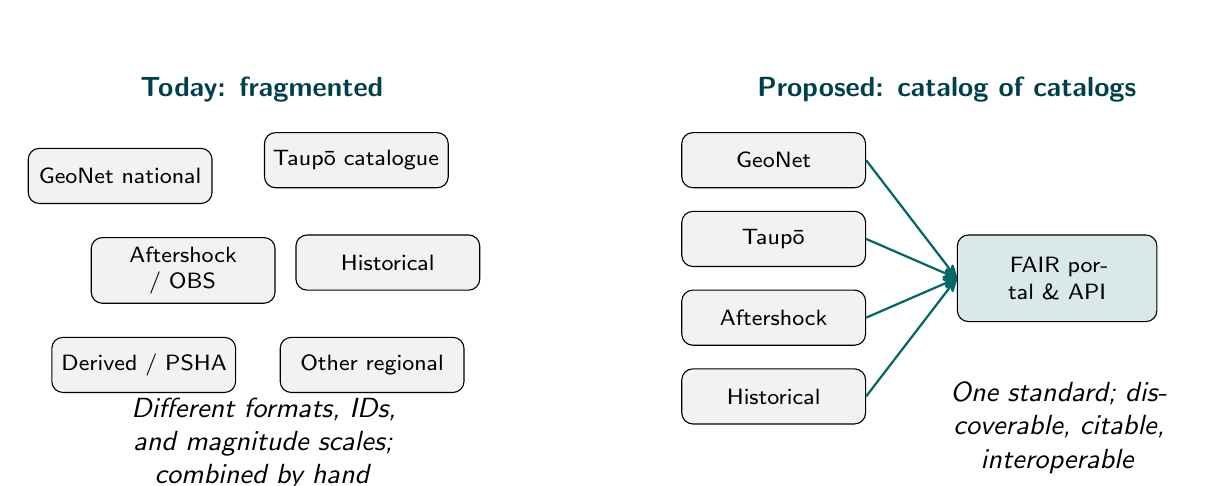
\begin{tikzpicture}[font=\footnotesize, >={Stealth[round]},
  cat/.style={draw, rounded corners, fill=gray!10, align=center, minimum height=0.7cm, text width=2.1cm},
  hub/.style={draw, rounded corners, fill=tealgreen!15, align=center, minimum height=1.1cm, text width=2.3cm}]
% LEFT: fragmented
\node[font=\bfseries, text=midnightgreen] at (2.0,4.6) {Today: fragmented};
\node[cat] at (0.2,3.5) {GeoNet national};
\node[cat] at (3.2,3.7) {Taup\=o catalogue};
\node[cat] at (1.0,2.3) {Aftershock / OBS};
\node[cat] at (3.6,2.4) {Historical};
\node[cat] at (0.5,1.1) {Derived / PSHA};
\node[cat] at (3.4,1.1) {Other regional};
\node[align=center, text width=4.3cm, font=\itshape] at (2.0,0.1) {Different formats, IDs, and magnitude scales; combined by hand};
% RIGHT: unified
\begin{scope}[xshift=8.5cm]
\node[font=\bfseries, text=midnightgreen] at (2.2,4.6) {Proposed: catalog of catalogs};
\node[cat] (g) at (0.0,3.7) {GeoNet};
\node[cat] (t) at (0.0,2.7) {Taup\=o};
\node[cat] (a) at (0.0,1.7) {Aftershock};
\node[cat] (h) at (0.0,0.7) {Historical};
\node[hub] (H) at (3.6,2.2) {FAIR portal \& API};
\foreach \n in {g,t,a,h} {\draw[->,thick,color=tealgreen] (\n.east) -- (H.west);}
\node[align=center, text width=3.4cm, font=\itshape] at (3.6,0.3) {One standard; discoverable, citable, interoperable};
\end{scope}
\end{tikzpicture}}
\caption{The problem and the opportunity. Today, New Zealand's earthquake catalogs are developed independently and combined manually. The proposed framework adds a coordinating layer that makes them interoperable through shared standards, a common portal, and a programmatic API --- complementing GeoNet rather than replacing it.}
\label{fig:fragmented}
\end{figure}

\section{The Current Landscape and International Benchmark}
\label{sec:landscape}
New Zealand's earthquake data ecosystem comprises several catalog types that serve different purposes. The \textbf{national operational catalog}, maintained through GeoNet by Earth Sciences New Zealand (ESNZ; formerly GNS Science), provides consistent coverage and open access since the 1930s \citep{GeoNetEqCatalogue, GeoNetFDSN, gns_neid}; its gaps are evolving metadata conventions, mixed magnitude types, spatially variable location quality \citep{WarrenSmith2025}, and limited exposure of detailed processing fields. \textbf{Regional and volcano-specific catalogs} add high-resolution detail using dense networks or specialised methods \citep{Illsley2025} but are often not interoperable with national standards. \textbf{Temporary deployment} catalogs are valuable yet not routinely discoverable. \textbf{Historical, derived, and synthetic} catalogs complement the instrumental era but, without formal versioning, identifiers, and processing documentation, are difficult to reuse or compare \citep{NSHM2022BSSA}. In short: strengths in local precision and national consistency; gaps in completeness through time and space, processing consistency, magnitude/depth scales, metadata, transparency, and access to legacy and temporary data.

Mature international systems show what ``good'' looks like: the USGS Advanced National Seismic System Comprehensive Earthquake Catalog (ComCat) federates 100+ networks \citep{usgs_comcat}; the Swiss Seismological Service couples a dense network with cross-border data \citep{sed_report}; the European-Mediterranean Seismological Centre (EMSC) and the International Seismological Centre (ISC) aggregate across many agencies \citep{emsc_webservices, isc_data_collection}; and EPOS provides standardised FAIR services across Europe \citep{EPOSSeisTCS}. These systems share common standards --- notably the International Federation of Digital Seismograph Networks (FDSN) web services and the QuakeML data format --- which New Zealand already supports. Appendix~\ref{app:international} summarises each. Table~\ref{tab:catalog_comparison} benchmarks New Zealand against these systems across ten dimensions and identifies the priority gaps: (1)~universal uncertainty reporting; (2)~formal version control with Digital Object Identifiers (DOIs) and changelogs; (3)~a cross-agency event-identifier mapping service; (4)~integration of historical and pre-instrumental data; and (5)~formal governance with dedicated funding.

\begin{landscape}
\begin{longtable}{@{}>{\raggedright\arraybackslash}p{3cm}>{\raggedright\arraybackslash}p{4cm}>{\raggedright\arraybackslash}p{3.5cm}>{\raggedright\arraybackslash}p{3.5cm}>{\raggedright\arraybackslash}p{3.5cm}@{}}
\caption{Comparison of NZ and International Earthquake Catalog Capabilities}
\label{tab:catalog_comparison} \\
\toprule
\textbf{Feature} & \textbf{New Zealand} & \textbf{USGS ComCat} & \textbf{Swiss SED / EPOS} & \textbf{Gaps \& Priorities} \\
\midrule
\endfirsthead

\multicolumn{5}{c}{\tablename\ \thetable{} -- \textit{continued}} \\
\toprule
\textbf{Feature} & \textbf{New Zealand} & \textbf{USGS ComCat} & \textbf{Swiss SED / EPOS} & \textbf{Gaps \& Priorities} \\
\midrule
\endhead

\midrule
\multicolumn{5}{r}{\textit{Continued on next page}} \\
\endfoot

\bottomrule
\endlastfoot

\textbf{Core parameters} &
Origin time, location, depth, magnitude, phase picks, station counts &
Hypocenter, magnitudes, phase data, moment tensors, macroseismic data \citep{usgs_comcat} &
Historical + instrumental events, uniform $M_w$, uncertainties, intensities \citep{sed_report} &
Lacks full uncertainty propagation for all events \\
\addlinespace

\textbf{Metadata \& provenance} &
Some document processing pipelines; incomplete or inconsistent across catalogs &
Maintains standards, data dictionaries, method documentation \citep{usgs_comcat} &
Adheres to FDSN, StationXML, QuakeML standards \citep{sed_report} &
Need consistent, centralised metadata policies \\
\addlinespace

\textbf{Versioning \& review} &
Rapid + review workflows; some reprocessing &
Versioned updates, multiple origins per event, revisions over time \citep{usgs_comcat} &
Unified access to evolving datasets, harmonisation &
Formalise version control (DOIs, changelogs) \\
\addlinespace

\textbf{Access \& APIs} &
Quake Search, FDSN, QuakeML, CSV/GeoJSON export &
FDSN API, GeoJSON/CSV feeds, search interfaces \citep{USGSFDSN} &
Integrated access to waveforms, parametric data via standards \citep{EPOSSeisTCS} &
Enhance federated discovery, cross-catalog queries \\
\addlinespace

\textbf{Historical data} &
Some pre-instrumental events with greater uncertainty &
Includes large historic events, variable completeness &
Centuries of data, macroseismic fields, uncertainties \citep{sed_report} &
Strengthen integration, metadata, uncertainty modelling \\
\addlinespace

\textbf{Uncertainty \& quality} &
Many provide estimates (location/magnitude error); not universal &
Quality metrics: RMS, station count, azimuthal gap \citep{usgs_comcat} &
Emphasises uncertainty, solution quality, EPOS standards \citep{sed_report} &
Universal uncertainty reporting needed \\
\addlinespace

\textbf{Multi-catalog linking} &
Mostly separate; limited cross-catalog mapping &
Aggregates many networks, links multiple origins per event \citep{usgs_comcat} &
Harmonised catalogs across Europe; cross-border exchange \citep{EPOSSeisTCS} &
Build Event ID mapping service, federated portal \\
\addlinespace

\textbf{Special products} &
Focal mechanisms, moment tensors, slow slip as standalone datasets &
Hosts moment tensors, additional products tied to events \citep{usgs_comcat} &
Integrates fault, slip, seismological products &
Better integrate special-purpose catalogs \\
\addlinespace

\textbf{Standards compliance} &
Supports FDSN/QuakeML; not all catalogs fully adhere &
FDSN and QuakeML in APIs and exports \citep{USGSFDSN} &
Full QuakeML, StationXML, FDSN compliance \citep{sed_report} &
Ensure full compliance across all catalogs \\
\addlinespace

\textbf{Governance \& sustainability} &
ESNZ/GeoNet or individual researchers; less formal structure &
Formal governance, funding, institutional roles (USGS/ANSS/NEIC) \citep{usgs_comcat} &
Robust institutional backing, cross-national coordination &
Establish formal governance, roles, funding \\

\end{longtable}
\end{landscape}

\section{A Community-Driven Process}
The framework was co-designed with the community. Two pre-conference workshops at the Geoscience Society of New Zealand annual meetings provided the primary engagement: a 2023 workshop framed needs and objectives, and a 2024 workshop reviewed progress and refined priorities \citep{GSNZWorkshop2023, GSNZWorkshop2024}. Participants spanned university researchers, GeoNet and Earth Sciences New Zealand staff, government agencies, and engineering and insurance users. Discussion was structured around eight thematic tables --- covering minimum catalog attributes, metadata and documentation, access and versioning, governance, and community priorities --- whose outcomes are summarised in Appendix~\ref{app:workshop}. Between workshops, a working group met regularly to draft standards, test integration pathways, and build a prototype portal.

\subsection{Prototype Portal: Proof of Concept}
\label{sec:prototype}
To ground the framework in a working system, the working group built a functional prototype portal and used it at the 2024 workshop to demonstrate ingestion, merge, export, and analytics workflows with representative New Zealand datasets. We describe it as a proof of concept rather than a validated production service: the capabilities below are implemented in the prototype, whereas the national framework in Section~\ref{sec:framework} is a proposal that, except where noted, is not yet implemented. The prototype demonstrates:
\begin{itemize}
\setlength{\itemsep}{1pt}
\item \textbf{Ingestion} of CSV/tab-delimited text (with automatic delimiter and date detection), JSON/GeoJSON variants, and QuakeML~1.2, with an alias-based field-mapping interface and direct, de-duplicating sync from GeoNet's FDSN Event service;
\item \textbf{Search and visualisation} --- spatial (bounding box, polygon, radius), time, magnitude, and depth filtering on an interactive map with event clustering, uncertainty ellipses, focal mechanisms, and station coverage;
\item \textbf{Merge and conflation} with four configurable strategies, conflict detection and logging, lineage tracking, and a pre-commit preview (Section~\ref{sec:merge});
\item \textbf{Analytics} --- Gutenberg-Richter $b$-value \citep{Aki1965}, completeness magnitude ($M_c$) \citep{Wiemer2000}, seismic-moment (energy) release, Gardner-Knopoff declustering \citep{GardnerKnopoff1974}, and multi-catalog magnitude-frequency comparison; and
\item \textbf{Multi-format export} (CSV, GeoJSON, KML, QuakeML~1.2), including version-specific exports.
\end{itemize}
Community feedback from the 2024 workshop informed refinements to the metadata schema, merge options, and quality-grading approach described next.

\section{The Proposed FAIR Framework}
\label{sec:framework}
The framework addresses the end-to-end lifecycle of catalog data; Figure~\ref{fig:architecture} summarises how its components fit together. This section describes the framework conceptually. Implementation-level detail --- API endpoints, access-control roles, field-level representations, and validation thresholds --- is collected in Appendix~\ref{app:spec} so that this section stays readable for a general audience.

\begin{figure}[H]
\centering
\resizebox{\textwidth}{!}{%
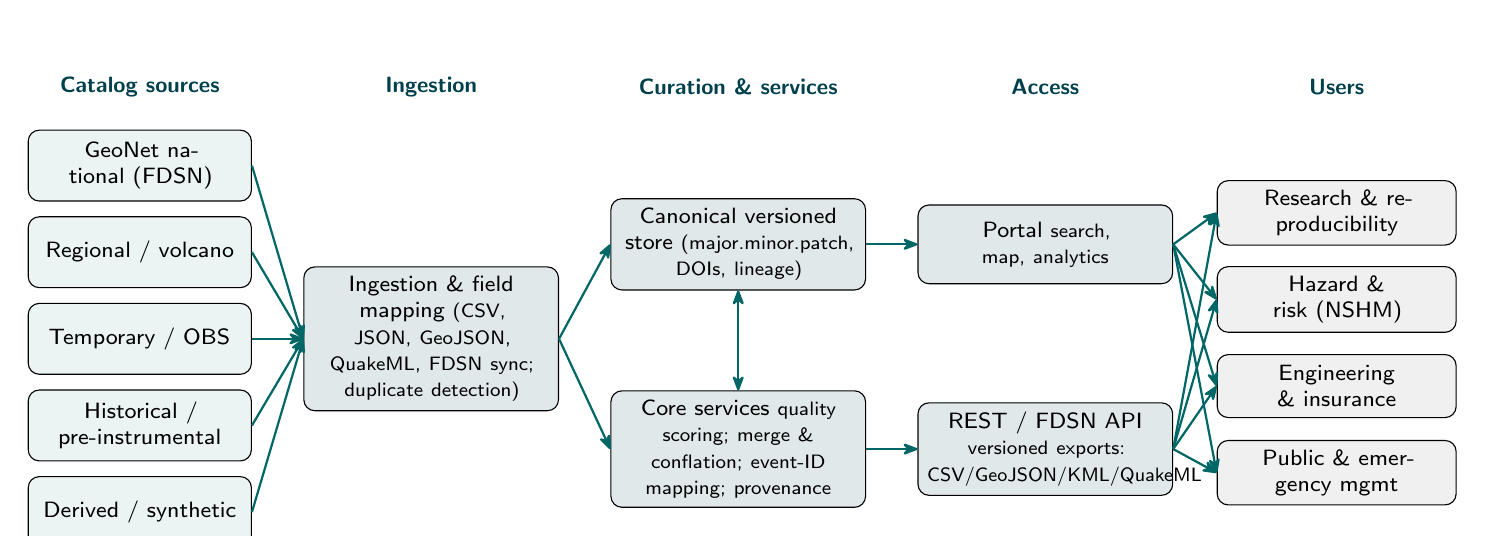
\begin{tikzpicture}[
  >={Stealth[round]},
  font=\footnotesize,
  src/.style={draw, rounded corners, fill=tealgreen!8, align=center, text width=2.6cm, minimum height=0.9cm},
  proc/.style={draw, rounded corners, fill=midnightgreen!12, align=center, text width=3.0cm, minimum height=1.0cm},
  cons/.style={draw, rounded corners, fill=gray!12, align=center, text width=2.8cm, minimum height=0.8cm},
  hdr/.style={font=\footnotesize\bfseries, text=midnightgreen},
  arr/.style={->, thick, color=tealgreen}
]
% Sources
\node[src] (s1) at (0,4.0) {GeoNet national (FDSN)};
\node[src] (s2) at (0,2.9) {Regional / volcano};
\node[src] (s3) at (0,1.8) {Temporary / OBS};
\node[src] (s4) at (0,0.7) {Historical / pre-instrumental};
\node[src] (s5) at (0,-0.4) {Derived / synthetic};
\node[hdr] at (0,5.0) {Catalog sources};
% Ingestion
\node[proc] (ing) at (3.7,1.8) {Ingestion \& field mapping {\scriptsize (CSV, JSON, GeoJSON, QuakeML, FDSN sync; duplicate detection)}};
\node[hdr] at (3.7,5.0) {Ingestion};
% Store + services
\node[proc] (store) at (7.6,3.0) {Canonical versioned store {\scriptsize (major.minor.patch, DOIs, lineage)}};
\node[proc] (svc) at (7.6,0.4) {Core services {\scriptsize quality scoring; merge \& conflation; event-ID mapping; provenance}};
\node[hdr] at (7.6,5.0) {Curation \& services};
% Access
\node[proc] (portal) at (11.5,3.0) {Portal {\scriptsize search, map, analytics}};
\node[proc] (api) at (11.5,0.4) {REST / FDSN API {\scriptsize versioned exports: CSV/GeoJSON/KML/QuakeML}};
\node[hdr] at (11.5,5.0) {Access};
% Consumers
\node[cons] (c1) at (15.2,3.4) {Research \& reproducibility};
\node[cons] (c2) at (15.2,2.3) {Hazard \& risk (NSHM)};
\node[cons] (c3) at (15.2,1.2) {Engineering \& insurance};
\node[cons] (c4) at (15.2,0.1) {Public \& emergency mgmt};
\node[hdr] at (15.2,5.0) {Users};
% arrows
\foreach \s in {s1,s2,s3,s4,s5} {\draw[arr] (\s.east) -- (ing.west);}
\draw[arr] (ing.east) -- (store.west);
\draw[arr] (ing.east) -- (svc.west);
\draw[arr,<->] (store) -- (svc);
\draw[arr] (store.east) -- (portal.west);
\draw[arr] (svc.east) -- (api.west);
\foreach \c in {c1,c2,c3,c4} {\draw[arr] (portal.east) -- (\c.west); \draw[arr] (api.east) -- (\c.west);}
\end{tikzpicture}%
}
\caption{End-to-end architecture of the proposed framework. Heterogeneous catalog sources are ingested and mapped to a canonical, versioned store; curation services (quality scoring, merge and conflation, event-identifier mapping, and provenance) feed a portal and a programmatic API that serve research, hazard, engineering, and public users. Capabilities identified as implemented in Section~\ref{sec:prototype} are exercised end-to-end by the prototype.}
\label{fig:architecture}
\end{figure}

\subsection{Metadata Standards and a Shared Lexicon}
A core metadata profile aligned with QuakeML and FDSN conventions captures identifiers, origin parameters with uncertainties, magnitude types with errors, detection and quality metrics, methodology descriptors, event classification, and catalog-level metadata \citep{QuakeML, GeoNetFDSN, USGSFDSN}. Required versus recommended fields are distinguished to balance utility against effort; the full field hierarchy is given in Table~\ref{tab:metadata_fields} (Appendix~\ref{app:spec}). A controlled vocabulary standardises magnitude types, event classifications, phase names and quality codes, units and formats, and dataset naming, improving interpretability and filtering across catalogs \citep{QuakeML, EventTypeNotes}.

\subsection{Interoperability: Programmatic Access and Cross-Catalog Identifiers}
A unified API provides machine-readable access across catalogs, returning CSV, GeoJSON, and QuakeML, with bulk downloads of versioned datasets to support reproducible research; it builds on existing GeoNet interfaces and standards \citep{GeoNetAPI, GeoNetFDSN, QuakeML}. The endpoint design is given in Appendix~\ref{app:spec}.

A persistent interoperability challenge is that the same earthquake carries different public identifiers across agencies --- a New Zealand event may appear as a GeoNet Public ID, a USGS event code, and an ISC event number --- so researchers aggregating sources must de-duplicate by hand. The framework includes an event-identity mapping service that maintains cross-agency equivalences, matched using configurable spatial, temporal, and magnitude thresholds (illustratively, separation $<$\,20\,km, time offset $<$\,30\,s, magnitude difference $<$\,0.5). These values are deliberately permissive to absorb differing location procedures; because wide windows can group genuinely distinct events in dense aftershock sequences, thresholds are configurable per source and ambiguous matches are flagged for expert review rather than merged automatically. The service aligns with the approach used by EMSC \citep{emsc_webservices} and extends it to the New Zealand context.

\subsection{Catalog Merge and Conflation}
\label{sec:merge}
Catalog conflation --- combining events from multiple independent catalogs into a unified view --- is a central operation. The framework specifies four merge strategies, all implemented in the prototype (Section~\ref{sec:prototype}); users choose by scientific objective:
\begin{itemize}
  \item \textbf{Priority-weighted}: a nominated agency's solution is preferred; others are recorded as alternatives.
  \item \textbf{Uncertainty-weighted average}: location, time, and magnitude are an inverse-variance-weighted mean across solutions.
  \item \textbf{Quality-based}: the highest quality-scored solution (Section~\ref{sec:quality}) is retained.
  \item \textbf{Complete-event}: the solution with the most populated recommended fields is retained.
\end{itemize}
Conflicts are detected and logged when solutions disagree beyond configurable thresholds (spatial separation, temporal offset, magnitude difference, depth range, network mismatch). Each merged event retains explicit lineage to its source events and the configuration used, enabling full audit and reproducibility; a dry-run preview returns conflict statistics without committing a new version. Table~\ref{tab:merge_example} shows a worked example.

\begin{table}[H]
\centering
\small
\caption{Worked example: uncertainty-weighted merge of one event reported by two agencies (illustrative values).}
\label{tab:merge_example}
\setlength{\tabcolsep}{5pt}
\renewcommand{\arraystretch}{1.15}
\begin{tabular}{p{3.1cm} p{3.1cm} p{3.1cm} p{3.5cm}}
\toprule
\textbf{Field} & \textbf{Source A (GeoNet)} & \textbf{Source B (USGS)} & \textbf{Merged (uncertainty-weighted)} \\
\midrule
Event identifier & 2016p858000 & us1000778i & merged-0001 (lineage to A, B) \\
Origin time (s past 11:02:00 UTC) & 56.3 $\pm$\,0.5 & 56.7 $\pm$\,0.8 & 56.4 $\pm$\,0.4 \\
Latitude (°) & $-42.737$ & $-42.740$ & $-42.738$ \\
Longitude (°) & 173.054 & 173.100 & 173.061 \\
Depth (km) & 15.1 $\pm$\,2.0 & 15.0 $\pm$\,4.0 & 15.1 $\pm$\,1.8 \\
Magnitude ($M_w$) & 7.8 $\pm$\,0.1 & 7.8 $\pm$\,0.1 & 7.8 $\pm$\,0.07 \\
Horizontal unc. (km) & 1.5 & 3.0 & 1.3 \\
\bottomrule
\end{tabular}
\end{table}

\subsection{Data Quality Assessment}
\label{sec:quality}
A standardised, transparent quality score supports informed reuse decisions, building on established practice for assessing catalog completeness and quality \citep{Woessner2005}. Quality is assessed across five dimensions: \textbf{completeness} (fraction of required/recommended fields populated), \textbf{accuracy} (internal consistency checks), \textbf{reliability} (reviewed-vs-automatic proportion, station count, azimuthal gap, phase count), \textbf{consistency} (temporal ordering, duplicate absence, cross-field agreement), and \textbf{traceability} (processing documentation, contact, version/publication links). An overall score (0--100) is a weighted sum (illustratively 40/20/15/15/10\,\%) mapping to the grade bands in Table~\ref{tab:quality_grades}. These weights and bands are an illustrative starting point, not an empirically calibrated standard: they should be tuned by the community against representative New Zealand catalogs, and both are configurable. The detailed automated checks and the full eight-band scheme are given in Appendix~\ref{app:spec}; flagged statistical outliers are annotated for caution rather than removed automatically.

\begin{table}[H]
\centering
\small
\caption{Quality Grade Bands and Recommended Use (illustrative; subject to community calibration; full scheme in Appendix~\ref{app:spec})}
\label{tab:quality_grades}
\setlength{\tabcolsep}{5pt}
\renewcommand{\arraystretch}{1.15}
\begin{tabular}{p{1.6cm} p{2cm} p{8.4cm}}
\toprule
\textbf{Grade} & \textbf{Score} & \textbf{Interpretation and recommended use} \\
\midrule
A & 85--100 & Suitable for hazard modelling and quantitative analysis. \\
B & 65--84  & Acceptable; document limitations or supplement metadata. \\
C & 45--64  & Poor; expert review recommended before quantitative use. \\
D/F & $<$45 & Minimal utility; discovery or illustrative purposes only. \\
\bottomrule
\end{tabular}
\end{table}

\subsection{Versioning, Persistent Identifiers, and Provenance}
Every catalog release carries a version, timestamp, and changelog, and all versions remain accessible for reproducibility. The framework uses a three-level \textsc{major.minor.patch} scheme (worked examples in Table~\ref{tab:versioning}, Appendix~\ref{app:spec}): \emph{major} increments alter event parameters, \emph{minor} increments add events or optional fields, and \emph{patch} increments touch only metadata or documentation.

Persistent identifiers make those releases citable. The catalog series carries a single concept DOI, and each major and minor release --- the changes that affect citable content --- receives its own version DOI \citep{DataCiteVersioning}; patch releases update the existing record without a new DOI, and frequent minor releases may be batched (for example, quarterly) to avoid identifier proliferation. A machine-readable changelog accompanies every release, so a researcher can cite the exact data state used in a study and a reviewer can see what changed between versions.

Processing steps (detection, picking, location, velocity models, magnitude calibration) and provenance are documented following a consistent model of entities, activities, and agents, with software version and execution date as minimum requirements \citep{PROVO}. Uncertainties for time, location, and magnitude are reported as standard deviations (with confidence-ellipse parameters where anisotropic) and always carry the magnitude type code; events without quantified uncertainties are flagged, and historical events may carry a qualitative confidence class (e.g.\ ``well-constrained'', ``felt-only''). Field-level representations are specified in Appendix~\ref{app:spec}.

\subsection{Special Catalog Types}
Different catalog types need adapted handling to preserve scientific value. In brief: regional research catalogs are ingested as distinct, separately versioned catalogs and cross-referenced --- not silently merged --- with the national catalog, because different processing assumptions can introduce systematic biases; temporary deployments are labelled with their time window and station geometry; historical and pre-instrumental catalogs use qualitative confidence classes and macroseismic intensity fields (Modified Mercalli or EMS-98, \citealp{Grunthal1998}) and form a distinct collection; and derived and synthetic catalogs carry explicit provenance to their sources. Appendix~\ref{app:spec} gives the detailed handling.

\subsection{Licensing and Access; FAIR Compliance Indicators}
To support FAIR reusability, every dataset and metadata record should carry an explicit, machine-readable license \citep{FAIRPrinciples2016, GOFAIR}; for government-funded baseline products a default open license aligned with New Zealand Government Open Access and Licensing (NZGOAL) guidance is recommended, with documented exceptions for embargoed, sensitive, or culturally restricted data \citep{NZGOAL2022}. Access is governed by a role-based model with catalog-level public/registered/restricted designations and, where needed, field-level masking of culturally sensitive locations; all write operations are audited. These mechanisms are detailed in Appendix~\ref{app:spec}. Progress should be tracked against a FAIR compliance matrix that maps each FAIR sub-principle (F1--F4, A1--A2, I1--I3, R1.1--R1.3) to a framework mechanism and a measurable, annually reported indicator --- for example, the percentage of catalogs with a resolvable DOI (F1), mean metadata-completeness (F2), API uptime (A1), and the percentage carrying a machine-readable license (R1.1). The full matrix is given in Table~\ref{tab:fair_matrix} (Appendix~\ref{app:spec}).

\subsection{Aotearoa New Zealand Data Governance: FAIR with CARE}
\label{sec:care}
In Aotearoa New Zealand the framework must be implemented consistently with both FAIR and the CARE Principles for Indigenous Data Governance, so that stewardship recognises Indigenous rights, authority, and benefit alongside openness \citep{CAREPrinciples2020}. For catalogs incorporating m\=atauranga-informed interpretations, iwi-relevant records, or sensitive contextual information, governance processes should document appropriate access conditions, attribution, and engagement pathways. The data-level access controls described above (Appendix~\ref{app:spec}) provide one technical mechanism to restrict or mask sensitive fields --- but they are only a mechanism: the appropriate conditions must be determined \emph{with}, not \emph{for}, iwi and hap\=u, who should be engaged as partners and decision-makers from the outset rather than consulted after the design is fixed. Accordingly, the Steering Committee (Section~\ref{sec:steering}) should include representation from relevant M\=aori communities and data-sovereignty advocates, so that CARE is operationalised rather than aspirational.

\section{Implementation: Governance, Roadmap, and Funding}
\label{sec:implementation}

\subsection{Governance, Roles, and Responsibilities}
\subsubsection{Steering Committee}
\label{sec:steering}
A Steering Committee provides strategic oversight and ensures community ownership. Membership should include Earth Sciences New Zealand, at least two universities with active seismology programmes, a government user (e.g.\ the National Emergency Management Agency), an engineering or insurance representative, an Indigenous data-sovereignty advocate, and an international advisor from a peer organisation (e.g.\ ISC, EMSC, or GFZ). It meets at least quarterly with defined decision-making processes and staggered three-year terms. The Committee approves new data sources for ingestion, ratifies versioning decisions affecting the national record, oversees international partnerships (e.g.\ alignment with EPOS), and commissions annual reporting against FAIR compliance indicators.

\subsubsection{Data Stewardship Team}
\label{sec:steward}
A Data Stewardship Team led by Earth Sciences New Zealand handles day-to-day operations: a Data Stewardship Lead, Data Managers (ingestion, metadata curation, quality review), a Software Engineer (API, infrastructure, security), and a User Support Analyst. External researchers may also submit catalogs through a defined contribution process (Section~\ref{sec:contribution}). These governance roles (contributor, reviewer, maintainer, steward) are distinct from the portal's technical access roles defined in Appendix~\ref{app:spec}.

\subsubsection{Catalog Contribution Process}
\label{sec:contribution}
External researchers and institutions may submit catalogs for inclusion. Submissions require: catalog name and description, responsible institution and contact, time period and geographic coverage, event count and magnitude range, format and metadata documentation, and a declared license. A two-stage review process applies: technical QC (format validity, completeness score, duplicate check) followed by scientific peer review (methods assessment, comparison with existing catalogs). The expected review timeline is four to eight weeks, with written feedback provided regardless of outcome. Approved catalogs are assigned a DOI and version record.

\subsubsection{Success Metrics and Annual Reporting}
Progress should be measured annually against indicators including: number of catalogs ingested; total event count and geographic coverage; proportion of catalogs at quality grade~A or above; API uptime (target 99.5\%); registered users; downloads and API queries; and peer-reviewed publications citing the platform or a versioned catalog DOI. Reporting against the FAIR sub-principle indicators (Table~\ref{tab:fair_matrix}) should also be included, and annual reports published openly. Illustrative two-year targets: the full GeoNet national catalog (well over one million events) plus 20 or more additional regional, temporary, and historical catalogs accessible through one interface; 200 or more registered users across the research, engineering, and agency communities; 10 or more research outputs citing a versioned catalog DOI; and API availability exceeding 99\%. These are indicative planning targets, not commitments, and should be revisited once the service is established.

\subsection{Roadmap}
Development proceeds in four phases (Figure~\ref{fig:roadmap}): planning and mobilisation; prototyping and pilot integration; full-scale implementation and public launch; and sustained operation as a national core service with annual review and FAIR compliance reporting.

\begin{figure}[H]
\centering
\resizebox{\textwidth}{!}{%
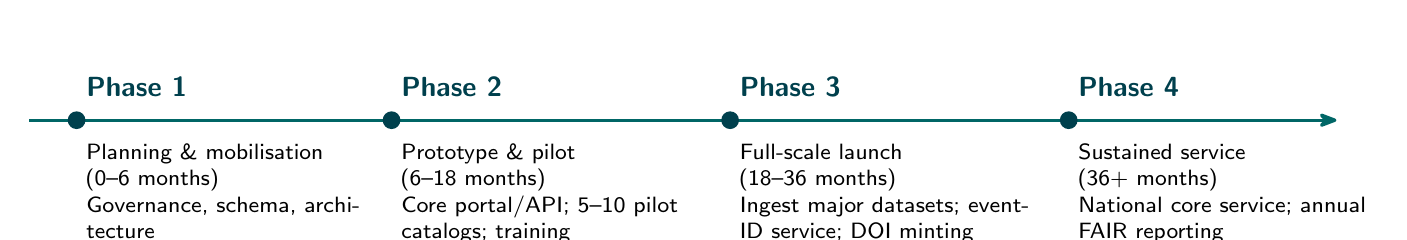
\begin{tikzpicture}[font=\footnotesize, >={Stealth[round]}]
\draw[->, very thick, color=tealgreen] (-0.3,0) -- (16.3,0);
\foreach \x/\t/\d in {%
  0.3/{Phase 1}/{Planning \& mobilisation\\(0--6 months)\\Governance, schema, architecture},
  4.3/{Phase 2}/{Prototype \& pilot\\(6--18 months)\\Core portal/API; 5--10 pilot catalogs; training},
  8.6/{Phase 3}/{Full-scale launch\\(18--36 months)\\Ingest major datasets; event-ID service; DOI minting},
  12.9/{Phase 4}/{Sustained service\\(36+ months)\\National core service; annual FAIR reporting}} {
  \fill[midnightgreen] (\x,0) circle (3.2pt);
  \node[anchor=south west, text=midnightgreen, font=\bfseries] at (\x,0.18) {\t};
  \node[anchor=north west, align=left, text width=3.7cm] at (\x,-0.18) {\d};
}
\end{tikzpicture}}
\caption{Indicative four-phase roadmap from planning to a sustained national service.}
\label{fig:roadmap}
\end{figure}

\subsection{Funding and Resourcing}
Indicative resourcing for a mature service is on the order of three to four full-time-equivalent (FTE) staff (Section~\ref{sec:steward}), together with cloud or on-premises infrastructure for storage, compute, and backup, and recurring DOI registration fees. A realistic path begins with a smaller team during Phases~1--2 and scales to the full complement at Phase~3. The figures here are indicative of scale, not costed estimates; precise budgets should be developed with host institutions and pursued through research-infrastructure programmes and operational budgets.

\section{Benefits by Stakeholder}
A coordinated, FAIR-and-CARE catalog capability delivers concrete, audience-specific value:
\begin{itemize}
\setlength{\itemsep}{2pt}
\item \textbf{Researchers} gain discoverable, citable, version-pinned datasets and ready cross-catalog comparison, making studies faster to run and genuinely reproducible.
\item \textbf{Hazard and risk modellers} (e.g.\ the National Seismic Hazard Model) get comparable, documented inputs with consistent magnitudes and uncertainties, reducing the bespoke harmonisation that the 2022 NSHM required \citep{NSHM2022BSSA}.
\item \textbf{Engineering and insurance} users obtain trusted, traceable inputs with explicit quality grades and licences, supporting defensible design and risk decisions.
\item \textbf{Emergency management and the public} benefit from clearer, better-documented event information and a single authoritative point of discovery.
\item \textbf{Iwi and hap\=u} are engaged as partners in governance, with technical mechanisms (access conditions, attribution, masking) that operationalise CARE.
\item \textbf{The national system} reduces duplication, preserves at-risk legacy and temporary datasets, and aligns New Zealand with international best practice \citep{EPOSSeisTCS}.
\end{itemize}

\section{Risks and Anticipated Questions}
We anticipate, and address, the main objections to this proposal:
\begin{itemize}
\setlength{\itemsep}{2pt}
\item \textbf{``Isn't this duplicating GeoNet?''} No. The framework is an aggregation and curation layer over GeoNet and the many catalogs outside it; GeoNet remains the authoritative operational source and a primary data provider (Figure~\ref{fig:architecture}).
\item \textbf{``Who pays once the establishment funding ends?''} Long-term sustainability is the reason for the governance and funding model in Section~\ref{sec:implementation}: a hosted national core service with a small standing team, not a project that ends with a grant.
\item \textbf{``What if researchers don't contribute their catalogs?''} The contribution process is low-friction and offers tangible incentives --- DOIs, citations, increased visibility, and quality feedback --- and the system delivers value from GeoNet and pilot catalogs from day one.
\item \textbf{``Why not just use EPOS, ISC, or ComCat?''} Those systems are complementary and the framework is designed to interoperate with them, but none curates New Zealand's regional, temporary, and historical catalogs or addresses CARE obligations; a national capability is still required.
\item \textbf{``Will standardisation flatten legitimate scientific differences?''} No. Alternative solutions are preserved with lineage, regional catalogs are cross-referenced rather than silently merged, and merge strategies are explicit and reproducible.
\end{itemize}

\section{Conclusion and Call to Action}
New Zealand has the data, the expertise, and a clear community mandate to make its earthquake catalogs FAIR; what is missing is a coordinating framework and the governance to sustain it. This white paper has set out that framework, benchmarked it against international practice, and demonstrated its feasibility through a working prototype. The remaining step is collective commitment.

We invite GeoNet and Earth Sciences New Zealand, universities, government agencies, iwi and hap\=u partners, and the engineering and insurance sectors to:
\begin{enumerate}
\setlength{\itemsep}{1pt}
\item endorse the metadata, lexicon, versioning, and quality standards proposed here as a shared national baseline;
\item commit to establishing the Steering Committee and Data Stewardship Team (Section~\ref{sec:steering}), with representation that operationalises both FAIR and CARE; and
\item support a multi-year funding case to move from prototype to a sustained national service.
\end{enumerate}
We welcome feedback on this draft and expressions of interest in participating in the governance and catalog-contribution processes described above. Comments may be directed to the corresponding author.

\section*{Data and Code Availability}
\addcontentsline{toc}{section}{Data and Code Availability}
In keeping with the FAIR principles it advocates, the material supporting this white paper is intended to be openly available. The prototype portal source code, the canonical metadata schema, and the controlled parameter lexicon are to be released under an open license at \texttt{[repository URL to be inserted]}, and a citable version of this document will be assigned a DOI (\texttt{[DOI to be inserted]}). The earthquake catalogs used as examples are available from their respective providers: the GeoNet national catalog \citep{GeoNetEqCatalogue}, USGS ComCat \citep{usgs_comcat}, and the Swiss Seismological Service \citep{sed_report}.

\section*{Acknowledgements}
We thank participants in the 2023 and 2024 workshops for their contributions, and colleagues across Earth Sciences New Zealand and partner universities for their ongoing input to this framework.

\textbf{Funding.} [Funding sources and grant numbers to be inserted.]

\textbf{Author contributions.} [Author contribution statement to be inserted.]


\appendix
\section{International Benchmark Detail}
\label{app:international}
This appendix expands the summary in Section~\ref{sec:landscape} and Table~\ref{tab:catalog_comparison}.

\subsection{New Zealand (GeoNet)}
GeoNet maintains New Zealand's earthquake catalog as part of the National Earthquake Information Database, the central repository for NZ seismic events~\citep{gns_neid}. The catalog contains origin time, location, magnitude, and seismic phase data, with each event assigned a unique Public ID~\citep{GeoNetEqCatalogue}, spanning instrumentally recorded earthquakes (1930s--present) and historical events from oral/written records~\citep{gns_neid}. Data access includes Quake Search (CSV, GeoJSON, KML, GML)~\citep{GeoNetEqCatalogue} and services compliant with the International Federation of Digital Seismograph Networks (FDSN) and Web Feature Service (WFS) standards, delivering QuakeML with uncertainties, phase arrivals, and multiple magnitude determinations~\citep{GeoNetFDSN,GeoNetLocationInfo}. Completeness is approximately $M_L$ 1--2 in well-monitored regions (higher elsewhere and through time); location quality varies markedly with station coverage, as quantified by \citet{WarrenSmith2025}. A 2022 revision moved the catalog toward more consistent magnitude reporting nationwide~\citep{gns_neid}.

\subsection{United States (USGS ComCat)}
The United States Geological Survey (USGS) operates the federated Advanced National Seismic System (ANSS) Comprehensive Earthquake Catalog (ComCat), covering global earthquakes ($M$4.5+ complete globally; $M$1--2.5 in the US)~\citep{usgs_comcat}, accessed via the FDSN Event API with QuakeML, CSV/GeoJSON/KML, and real-time GeoJSON feeds~\citep{USGSFDSN}. Entries include quality metrics (stations used, azimuthal gap, RMS residuals) and magnitude uncertainty; ComCat integrates 100+ networks, stores multiple solutions per event with one preferred, and hosts products such as ShakeMap and crowdsourced intensity data~\citep{usgs_comcat}.

\subsection{Switzerland (SED)}
The Swiss Seismological Service (SED) maintains a high-quality catalog dating to 1879~\citep{sed_report}, with historical events to 250~AD. A dense network achieves $M_c$ 1.0--1.5 completeness; SED introduced updated magnitude scales ($M_{Lhc}$, 2020), employs 3D velocity models and relative relocation, and provides formal uncertainties via QuakeML since 2013~\citep{sed_report}. Data are accessible through FDSN web services, and cross-border collaboration integrates 60+ stations from France, Germany, Italy, and Austria~\citep{sed_report}. The ECOS project unified historical records into a homogenised database~\citep{ECOS09}.

\subsection{European and Global Aggregators}
The European-Mediterranean Seismological Centre (EMSC) operates the European Seismic Portal, aggregating data from multiple networks via FDSN-compliant services and providing multiple solutions and phase data~\citep{emsc_home,emsc_webservices}. The International Seismological Centre (ISC) archives global bulletin data from 130+ agencies, accepting multiple formats (Nordic, GSE, ISF, QuakeML)~\citep{isc_data_collection} with output in ISF or QuakeML~\citep{isc_bulletin}. Other agencies (the Japan Meteorological Agency, Geoscience Australia, and the European Integrated Data Archive) have adopted FDSN services, and major catalogs now share common standards for open, interoperable access~\citep{EPOSSeisTCS,QuakeML}.

\section{Draft Technical Specification}
\label{app:spec}
This appendix collects implementation-level detail referenced from Section~\ref{sec:framework}. It is indicative and intended to be refined during Phase~1.

\subsection{Metadata Field Hierarchy}
Table~\ref{tab:metadata_fields} gives the full catalog- and event-level metadata profile summarised in Section~\ref{sec:framework}, distinguishing required from recommended fields.

\begin{table}[H]
\centering
\small
\caption{Metadata Field Hierarchy for FAIR Catalog Records}
\label{tab:metadata_fields}
\setlength{\tabcolsep}{5pt}
\renewcommand{\arraystretch}{1.15}
\begin{tabular}{p{3.2cm} p{2cm} p{8cm}}
\toprule
\textbf{Field} & \textbf{Status} & \textbf{Description} \\
\midrule
\multicolumn{3}{l}{\textit{Catalog-level}} \\
\midrule
Persistent identifier & Required & DOI or equivalent resolvable identifier \\
Name, description & Required & Human-readable title and summary \\
Institution, contact & Required & Responsible party and contact details \\
Temporal coverage & Required & Start and end date of events \\
Geographic coverage & Required & Bounding box or region descriptor \\
Magnitude range & Required & Minimum and maximum magnitude \\
Event count & Required & Total number of events \\
License & Required & Machine-readable license identifier (e.g.\ CC-BY 4.0) \\
Processing summary & Required & High-level description of methods \\
Velocity model & Recommended & Reference to velocity model used \\
Location algorithm & Recommended & Software and version (e.g.\ NonLinLoc 7.0) \\
Magnitude calibration & Recommended & Scale definitions and calibration reference \\
Publication links & Recommended & DOIs of associated papers \\
\midrule
\multicolumn{3}{l}{\textit{Event-level}} \\
\midrule
Origin time & Required & UTC time (ISO 8601) \\
Latitude, longitude & Required & WGS84 decimal degrees \\
Depth & Required & Kilometres below sea level \\
Magnitude value \& type & Required & Value and scale code (e.g.\ $M_w$, $M_L$) \\
Origin time uncertainty & Recommended & Seconds (1$\sigma$) \\
Horizontal uncertainty & Recommended & Kilometres (1$\sigma$) \\
Vertical uncertainty & Recommended & Kilometres (1$\sigma$) \\
Magnitude uncertainty & Recommended & Standard deviation \\
Station count & Recommended & Number of stations used \\
Azimuthal gap & Recommended & Degrees \\
Phase count & Recommended & Number of phase picks used \\
RMS residual & Recommended & Seconds \\
Evaluation status & Recommended & ``automatic'' or ``reviewed'' \\
Event type & Recommended & QuakeML event type vocabulary \\
\bottomrule
\end{tabular}
\end{table}

\subsection{Versioning Scheme}
Table~\ref{tab:versioning} illustrates the version-increment triggers for the three-level \textsc{major.minor.patch} scheme described in Section~\ref{sec:framework}.

\begin{table}[H]
\centering
\small
\caption{Versioning Scheme: Examples of Version Increment Triggers}
\label{tab:versioning}
\setlength{\tabcolsep}{5pt}
\renewcommand{\arraystretch}{1.15}
\begin{tabular}{p{2cm} p{4cm} p{7cm}}
\toprule
\textbf{Version} & \textbf{Trigger} & \textbf{Example change} \\
\midrule
\textsc{major} & Event parameters changed & Reprocessing with new 3D velocity model; recalibration of magnitude scale; new location algorithm affecting systematic offsets \\
\textsc{minor} & New events or fields added & Ingestion of 500 additional aftershock events; addition of focal mechanism fields to existing events \\
\textsc{patch} & Metadata or documentation & Contact email updated; description clarified; deprecated field removed from catalog-level record \\
\bottomrule
\end{tabular}
\end{table}

\subsection{API Design}
A unified API follows REST conventions. Authentication uses token-based credentials for write operations; read operations on public catalogs are unauthenticated. Rate limiting protects service availability, and standard HTTP error codes with a consistent JSON error envelope enable reliable programmatic error handling. Output format is negotiated via the \texttt{Accept} header or a \texttt{format} query parameter, defaulting to GeoJSON for spatial queries and CSV for tabular exports; QuakeML output is generated from the canonical internal event model, preserving uncertainty fields, evaluation status, and magnitude type. Table~\ref{tab:api_endpoints} summarises the principal endpoint categories.

\begin{table}[H]
\centering
\small
\caption{Principal API Endpoint Categories}
\label{tab:api_endpoints}
\setlength{\tabcolsep}{5pt}
\renewcommand{\arraystretch}{1.15}
\begin{tabular}{p{3cm} p{4.5cm} p{5.5cm}}
\toprule
\textbf{Category} & \textbf{Operations} & \textbf{Notes} \\
\midrule
Catalogs & List, retrieve, create, update, delete & Metadata including bounds, event count, license \\
Events & List, spatial query, time-range, magnitude/depth filter & Pagination; supports GeoJSON, CSV, QuakeML output \\
Search & Cross-catalog full-text and parameter search & Returns ranked results across all accessible catalogs \\
Import & Upload file, sync from FDSN source, view history & Supports CSV, JSON, GeoJSON, QuakeML 1.2 \\
Merge & Preview, execute, retrieve conflict log & Dry-run mode returns statistics without committing \\
Export & Per-catalog or per-query download & CSV, GeoJSON, KML, QuakeML; version-specific \\
Versions & List versions, retrieve specific version & Version-specific event snapshots remain available indefinitely \\
\bottomrule
\end{tabular}
\end{table}

\subsection{Access Control and Audit}
Access to catalog data and portal operations is governed by a role-based model. Four \emph{technical} roles are defined (distinct from the governance roles of Section~\ref{sec:contribution}; a single individual may hold both):
\begin{itemize}
  \item \textbf{Administrator}: full access including user management, system configuration, and deletion of catalog records.
  \item \textbf{Editor}: can create and modify catalogs, import data, and initiate merge operations, but cannot manage users or alter system configuration.
  \item \textbf{Viewer}: can search, view, filter, and export catalogs to which they have been granted access, but cannot modify data.
  \item \textbf{Guest} (unauthenticated): can discover and download public catalogs; embargoed or restricted catalogs are not visible.
\end{itemize}
Role assignments are managed by Administrators and recorded in an audit log; a role-upgrade request workflow allows registered users to request elevated access.

\textbf{Data-level access control.}\label{sec:dataaccess} Each catalog carries one of three access designations: \textbf{public} (all, unauthenticated), \textbf{registered} (authenticated Viewers and above), or \textbf{restricted} (named individuals or groups). This supports time-limited embargoes (e.g.\ allowing a research group to work privately until a companion paper is published). Field-level masking may be applied where a catalog contains sensitive location information, such as event locations near culturally significant sites: coordinates may be spatially generalised or withheld for Guest and Viewer access while full precision is retained for authorised users, consistent with the CARE discussion in Section~\ref{sec:care}.

\textbf{Audit and compliance.} All write operations (catalog creation, import, merge, deletion) are recorded with the authenticated user identity, timestamp, and operation details; read access to restricted catalogs is similarly logged. Where usage agreements are attached to a catalog (for example, a requirement to cite a companion publication), the agreement is presented at download time and acceptance is recorded.

\subsection{Uncertainty Representation}
Origin location and time uncertainties are reported as standard deviations: \texttt{time\_uncertainty} (seconds), \texttt{horizontal\_uncertainty} (kilometres), and \texttt{depth\_uncertainty} (kilometres). Where horizontal uncertainty is anisotropic, the semi-major and semi-minor axes of the 68\% confidence ellipse and its azimuth are reported, mapping directly to QuakeML \texttt{OriginUncertainty} elements \citep{QuakeML}. Magnitude uncertainties are reported as the standard deviation on the stated scale, and the magnitude type code must always accompany the value. Events without quantified uncertainties carry a boolean \texttt{uncertainty\_available} field set to false; historical events may substitute a qualitative confidence class. When events are merged, uncertainty-weighted averaging combines standard deviations by inverse-variance weighting, while priority/quality strategies retain the selected solution's uncertainty and record alternatives; the merge log documents the strategy and resulting uncertainty.

\subsection{Quality Checks and Full Grade Scheme}
Representative automated checks include: events ordered chronologically; no future-dated events; depth within a physically plausible range for the region (e.g.\ $-5$ to 1000\,km, the negative bound allowing for events above the sea-level datum); magnitude within a plausible range for the declared region; uncertainty values non-negative and within parameter-specific sanity bounds (for example, horizontal uncertainty not exceeding the catalog's declared spatial extent, and magnitude uncertainty below a configurable ceiling such as 1.0 magnitude unit); no coordinate pair repeated for distinct events at an identical time; station count $\geq$\,5 for the event to be considered well-constrained; and azimuthal gap $<$\,180° for reliable depth estimates \citep{usgs_comcat}. Results are summarised as passed, warning, or failed. The full eight-band grade scheme underlying the summary in Table~\ref{tab:quality_grades} is given in Table~\ref{tab:quality_grades_full}.

\begin{table}[H]
\centering
\small
\caption{Full Quality Grade Thresholds and Recommended Use (illustrative; subject to community calibration)}
\label{tab:quality_grades_full}
\setlength{\tabcolsep}{5pt}
\renewcommand{\arraystretch}{1.15}
\begin{tabular}{p{1.5cm} p{2cm} p{8.5cm}}
\toprule
\textbf{Grade} & \textbf{Score} & \textbf{Interpretation and recommended use} \\
\midrule
A+ & 95--100 & Excellent. Publication-ready; suitable for hazard modelling and all quantitative analysis. \\
A  & 85--94  & Good. Suitable for most research and engineering applications. \\
B+ & 75--84  & Acceptable. Minor gaps; document limitations in methods sections. \\
B  & 65--74  & Fair. Notable gaps; consider supplementing with additional metadata. \\
C+ & 55--64  & Poor. Significant gaps; expert review recommended before quantitative use. \\
C  & 45--54  & Very poor. Limited utility for quantitative analysis. \\
D  & 35--44  & Minimal utility. Use only for discovery or illustrative purposes. \\
F  & $<$35   & Not recommended for quantitative analysis. \\
\bottomrule
\end{tabular}
\end{table}

\subsection{Special Catalog Type Handling}
\textbf{Regional research catalogs} produced with specialised methods (e.g.\ 3D velocity models, relative relocation, custom magnitude calibrations) are ingested as distinct catalogs with their own version records and DOIs; processing methods are documented in catalog-level metadata, and the portal provides cross-reference links between co-temporal events in regional and national catalogs with the spatial and magnitude offset reported. \textbf{Temporary deployment catalogs} are ingested with an explicit time window and a ``research'' or ``monitoring'' designation, with station-geometry metadata and links to relevant FDSN waveform services. \textbf{Historical and pre-instrumental catalogs} are accommodated through qualitative location confidence classes, macroseismic intensity fields (Modified Mercalli or EMS-98, \citealp{Grunthal1998}), narrative source-attribution fields, and separate quality thresholds, and are presented as a separate collection. \textbf{Derived and synthetic catalogs} carry mandatory provenance identifying source catalog(s), derivation method, parameters, and software, with explicit ``derivedFrom'' relations to source versions; synthetic catalogs are labelled as such.

\subsection{FAIR Compliance Matrix}
Table~\ref{tab:fair_matrix} gives the full mapping summarised in Section~\ref{sec:framework}: each FAIR sub-principle, the framework mechanism that addresses it, and a measurable indicator for annual reporting.

\begin{table}[H]
\centering
\small
\caption{Illustrative FAIR Compliance Matrix: Sub-Principle, Framework Mechanism, and Indicator}
\label{tab:fair_matrix}
\setlength{\tabcolsep}{5pt}
\renewcommand{\arraystretch}{1.15}
\begin{tabular}{p{1.2cm} p{5.3cm} p{6.0cm}}
\toprule
\textbf{Sub-pr.} & \textbf{Framework mechanism} & \textbf{Indicator} \\
\midrule
F1 & Persistent identifiers (DOIs) for catalogs; stable event identifiers & \% of catalogs with a resolvable DOI; \% of events with a stable ID \\
F2 & Rich metadata profile (catalog- and event-level) & Mean metadata-completeness score across catalogs \\
F3 & Metadata records embed the data identifier & \% of metadata records linking to their data identifier \\
F4 & Indexing in the searchable portal and discovery API & \% of catalogs indexed and discoverable \\
\addlinespace
A1 & Retrieval via FDSN/REST over HTTPS & API uptime; \% of catalogs retrievable by identifier \\
A1.1/A1.2 & Open, standard protocols; token auth only for write/restricted data & \% of read endpoints requiring no authentication \\
A2 & Metadata and version records retained after data withdrawal & \% of withdrawn datasets with surviving metadata \\
\addlinespace
I1 & QuakeML / FDSN standard representations & \% of catalogs available as valid QuakeML \\
I2 & Controlled parameter lexicon (magnitude, event, phase types) & \% of fields using controlled-vocabulary terms \\
I3 & Qualified cross-references (event-ID mapping, lineage links) & \% of merged events with recorded source lineage \\
\addlinespace
R1.1 & Machine-readable license on every record & \% of catalogs with a machine-readable license \\
R1.2 & PROV-based provenance (entities, activities, agents) & Mean provenance-completeness score \\
R1.3 & Conformance to FDSN/QuakeML community standards & \% of catalogs passing standards-compliance checks \\
\bottomrule
\end{tabular}
\end{table}

\section{Summary of Workshop Tables 1--8}
\label{app:workshop}
This appendix summarises the full set of workshop discussions captured across eight interactive tables. The content reflects community perspectives on minimum catalog attributes, metadata requirements, processing concerns, governance needs, and priorities for a national FAIR-aligned framework for earthquake catalogs in Aotearoa New Zealand.
\begin{table}[H]
\centering
\small
\caption{Summary of Key Themes from Workshop Tables 1--8}
\setlength{\tabcolsep}{6pt}
\renewcommand{\arraystretch}{1.15}
\begin{tabular}{p{3.2cm} p{11cm}}
\hline
\textbf{Theme} & \textbf{Key Points} \\
\hline

\textbf{Minimum Catalog Attributes} &
Phase picks; station metadata; velocity models (1D/3D); depths and magnitudes with uncertainties; completeness estimates; region of interest; unique IDs; focal mechanisms; processing history; detection and processing methods. \\[0.2cm]

\textbf{Metadata \& Documentation Needs} &
Clear methodology (location algorithm, velocity model, filters); solution provenance; waveform availability; descriptive summaries; parameter definitions; assumptions (point-source vs 2D/3D); embargo details; QC information; required README and DOI; multiple contacts. \\[0.2cm]

\textbf{Access \& Versioning} &
Raw data accessibility; open formats (CSV, QuakeML, FDSN); programmatic access (API); search by region, time, magnitude; support for multiple versions; backward/forward compatible formats; tracking of method changes; long-term storage of legacy releases. \\[0.2cm]

\textbf{Governance Needs} &
Defined roles (contributor, reviewer, maintainer); central catalog portal; consistent naming conventions; periodic updates; upload validation; framework transparency; responsibility for long-term stewardship. \\[0.2cm]

\textbf{Community Priorities} &
National catalog portal; common parameter lexicon; national 3D community velocity model; honest uncertainties; digitisation \& reprocessing of legacy data; cross-catalog interoperability; clear documentation for older datasets. \\[0.2cm]

\textbf{Concerns Raised} &
Inconsistent completeness; variable processing; missing metadata; uncertain magnitude/depth scales; ``black-box'' ML outputs; compatibility issues across regional/temporary catalogs; handling of unpublished datasets; need for quality flags and user warnings. \\[0.2cm]

\textbf{Desired Portal Features} &
Merge multiple catalogs; support subcatalogs; synthetic catalogs; geographic reference tools; method-based filtering; visualisation; minimum-requirements upload form; linkage among event, waveform, and station data. \\[0.2cm]

\textbf{What Users Liked} &
Simple form; unified access; clear uncertainty fields; reproducibility focus; increased awareness of catalog availability; prioritisation of essential fields. \\[0.2cm]

\textbf{Requested Improvements} &
More metadata fields and filters; better uncertainty representation; link with 2D/3D models; clarify naming/versioning; transparent ML integration; improved handling of old locations; inclusion of focal mechanisms and strong-motion connections. \\
\hline
\end{tabular}
\end{table}



\bibliographystyle{apalike}
\bibliography{catalogBib}

\end{document}
